% !TEX root = tracking.tex
\section{Offline Computation \label{sec:precomp}}
The offline computation begins with setting up a pursuit-evasion game \cite{Huang11, Chen17} between the tracking system and the planning system. 
In this game, the tracking system will try to ``capture" the planning system, while the planning system is doing everything it can to avoid capture. 
In reality the planner is typically not actively trying to avoid the tracking system, but this allows us to account for worst-case scenarios and more crucially, ensure that the TEB is \textit{trajectory-independent}. 
If both systems are acting optimally in this way, we want to determine the largest relative distance (based on some suitable metric) that may occur over time. 
This distance is the maximum possible tracking error between the two systems, and is captured by the value function obtained from solving the HJ VI \eqref{eq:HJVI}.

\subsection{Relative System Dynamics}
To determine the relative distance (or another error metric) that may occur over time, we must first define the relative system derived from the tracking and planning models. 
The individual dynamics are defined in Section \ref{sec:formulation}, equations (\ref{eq:tdyn}) and (\ref{eq:pdyn}). 
The relative system is obtained by fixing the planning model to the origin and finding the dynamics of the tracking model relative to the planning model.
Defining $\rstate$ to be the relative system state, we write

\begin{equation}
\label{eq:rstate}
\rstate = \rtrans(\tstate - \ptmat\pstate)
\end{equation}

\noindent where $\ptmat$ matches the common states of $\tstate$ and $\pstate$ by augmenting the state space of the planning model.
The relative system states $\rstate$ represent the tracking system states relative to the planning states.

The function $\rtrans$ is a nonlinear transform, usually either the identity function or a rotation, that facilitates simplification of the relative system dynamics to be of the form

\begin{equation}
\label{eq:rdyn}
\dot\rstate = \rdyn(\rstate, \tctrl, \pctrl, \dstb),
\end{equation}

\noindent which only depends on the relative system state $r$.
A transform $\rtrans$ that achieves the relative system dynamics in the form of \eqref{eq:rdyn} is not strictly needed and may not exist; however, in principle the theory we present can be easily adapted to this case, albeit at a cost of having a higher-dimensional relative system.
In this paper, we assume that a suitable $\rtrans$ is available so that the dimensionality of the relative system state space is at most that of the tracking model.

In addition, we define the error state $\estate$ to be the relative system state \textit{excluding} the absolute states of the tracking system, and the auxiliary states $\astate$ to be the relative system state \textit{excluding} the error state.
Hence, $\rstate = (\estate, \astate)$.

To be concrete, let the tracking model be a 5D car model, and the planning model be a 3D kinematic car model as follows:

\begin{equation}
\label{eq:5D_and_3D_dyn}
\dot \tstate = 
\begin{bmatrix}
\dot x\\
\dot y\\
\dot\theta\\
\dot v\\
\dot \omega
\end{bmatrix} =
\begin{bmatrix}
v \cos \theta + \dstb_x\\
v \sin \theta + \dstb_y\\
\omega \\
a + \dstb_a\\
\alpha + \dstb_\alpha
\end{bmatrix}, \quad
\dot \pstate = 
\begin{bmatrix}
\dot {\hat x}\\
\dot {\hat y}\\
\dot {\hat \theta}
\end{bmatrix}
=
\begin{bmatrix}
\hat v \cos \hat\theta\\
\hat v \sin \hat\theta\\
\hat \omega
\end{bmatrix},
\end{equation}

\noindent where $(x,y,\theta),(\hat x, \hat y, \hat\theta)$ represent the pose (position and heading) of the 5D and 3D car model respectively.
The speed and turn rate $(v, \omega)$ are states for the 5D model; for the 3D model the speed $\hat v$ is a constant, and the turn rate $\hat \omega$ is the control.
The control of the 5D model consists of the linear and angular acceleration, $(a, \alpha)$, and the disturbances are $(\dstb_x, \dstb_y, \dstb_a, \dstb_\alpha)$.

We define the relative system state to be $(x_r, y_r, \theta_r, v, \omega)$, such that the error state $\estate=(x_r, y_r, \theta_r)$ is the position and heading of the 5D model in the reference frame of the 3D model, and the auxiliary state $\astate = (v, \omega)$ represents the speed and turn rate of the 5D model.
The relative system state $\rstate = (\estate, \astate)$, tracking model state $\tstate$, and planning model state $\pstate$ are related through $\rtrans$ and $\ptmat$ as follows:

\begin{equation}\small
\label{eq:5D_and_3D_err_state}
\underbrace{
\begin{bmatrix}
x_r\\
y_r\\
\theta_r \\
v \\
\omega
\end{bmatrix}
}_\rstate
=
\underbrace{
\begin{bmatrix}
  \begin{bmatrix}
  \cos\hat\theta & \sin\hat\theta \\
  -\sin\hat\theta & \cos\hat\theta
  \end{bmatrix} & \mathbf{0_{2\times 3}} \\
  \mathbf{0_{3\times 2}} & \mathbf I_3
\end{bmatrix}
}_\rtrans
\Bigg(
\underbrace{
\begin{bmatrix}
x\\
y\\
\theta \\
v \\
\omega
\end{bmatrix}
}_\tstate -
\underbrace{
\begin{bmatrix}
\mathbf I_3 \\
\mathbf{0_{2\times 3}}
\end{bmatrix}
}_\ptmat
\underbrace{
\begin{bmatrix}
\hat x\\
\hat y \\
\hat \theta \\
\end{bmatrix}
}_\pstate
\Bigg),
\end{equation}

\noindent where $\mathbf 0, \mathbf I$ denote the zero and identity matrices of the indicated sizes.
Taking the time derivative, we obtain the following relative system dynamics:

\begin{equation}
\label{eq:5D_and_3D_rdyn}
\dot \rstate = 
\begin{bmatrix}
\dot \estate\\
\dot \astate
\end{bmatrix}
=
\begin{bmatrix}
\dot x_r\\
\dot y_r\\
\dot\theta_r\\
\dot v\\
\dot \omega
\end{bmatrix}
=
\begin{bmatrix}
- \hat v + v \cos \theta_r + \hat \omega y_r + \dstb_x\\
v \sin \theta_r - \hat \omega x_r + \dstb_y\\
\omega - \hat \omega \\
a + \dstb_a\\
\alpha + \dstb_\alpha
\end{bmatrix}.
\end{equation}

More examples of relative systems can be found in Sections \ref{sec:resultsRRT} and \ref{sec:resultsMPC}.

\subsection{Formalizing the Pursuit-Evasion Game}
Given the relative dynamics between the tracking system and the planning system, we would like to compute a guaranteed TEB between these systems. 
This is done by first defining a error function $\errfunc(\rstate)$ in the relative state space of the systems. 
One typical error function is distance to the origin, which corresponds to the tracking error in terms of Euclidean distance between the tracking and planning systems. 
This error function is shown in Fig. \ref{fig:vf_TEB:5D3D}. 
Of course, the error function can be defined in any desired manner, and involve planning state variables other than position.
For example, the error function, which corresponds to $\valfunc(\rstate, 0)$ in Fig. \ref{fig:vf_TEB:8D4D}, is defined in both position and velocity space; Fig. \ref{fig:vf_TEB_10D3D} shows yet another error function defined using the one-norm of the displacement between the two systems. 
In our pursuit-evasion game formulation, the tracking system tries to minimize this cost, while the planning system and any disturbances experienced by the tracking system try to do the opposite -- maximize.

\begin{figure}
  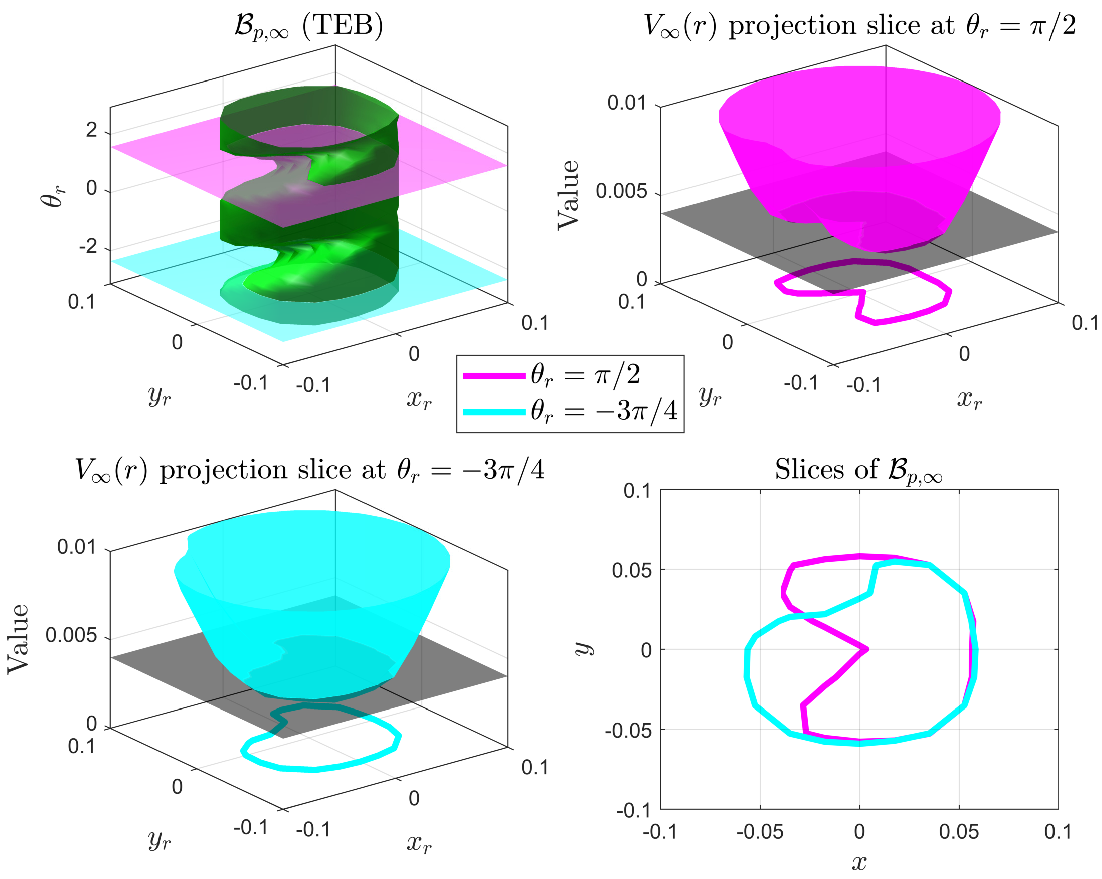
\includegraphics[width=\columnwidth]{fig/ti_valfunc_5d3d}
  \caption{Infinite time horizon TEB (top left), two slices of the value function at $\theta_r = \pi/2, -3\pi/4$ (top right, bottom left), and corresponding TEB slices (bottom right) for the 5D car tracking 3D Dubins car example in Section \ref{sec:reach_planner}.}
  \label{fig:vf_TEB:5D3D}  
\end{figure}

\begin{figure}
	\centering
  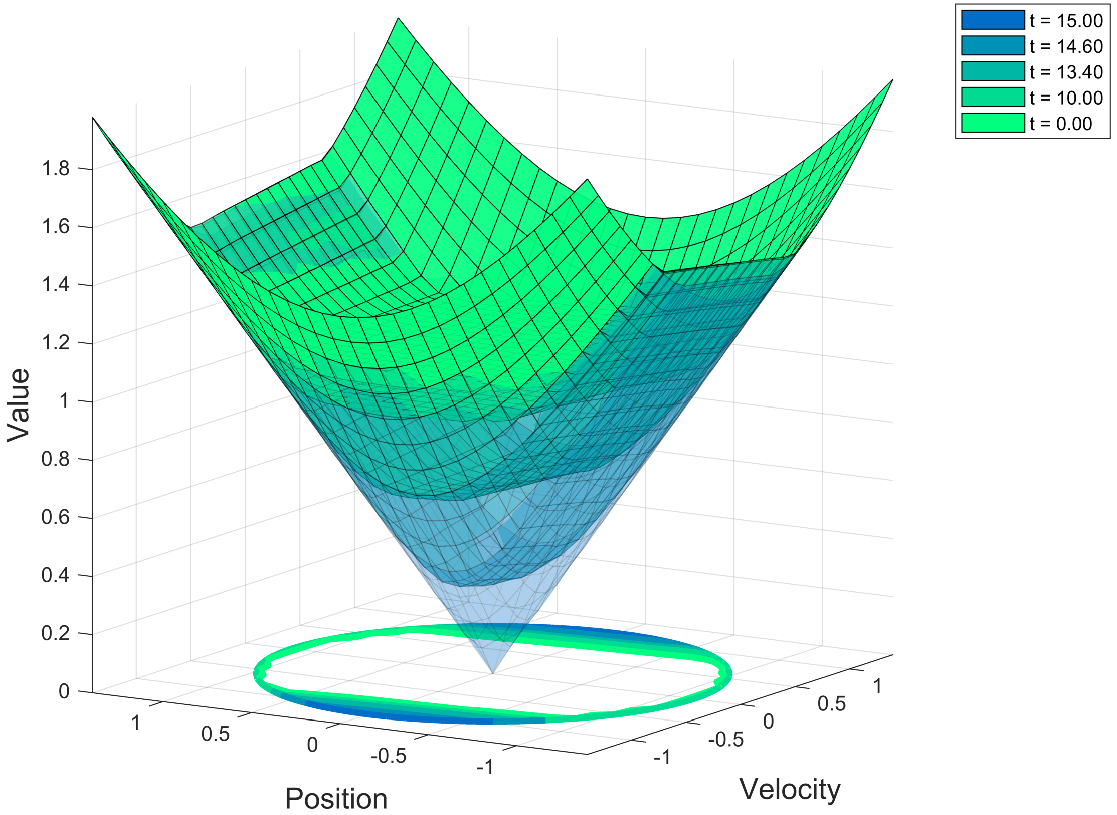
\includegraphics[width=\columnwidth]{fig/tv_valfunc}
  \caption{Finite time horizon value function (top) and TEBs (bottom) for the 8D quadrotor tracking 4D double integrator example in Section \ref{sec:resultsMPC}.}  
  \label{fig:vf_TEB:8D4D}
\end{figure} 

Before constructing the pursuit-evasion game we must first define the method each player must use for making decisions. 
We define a strategy for planning system as the mapping $\gamma_{\pstate} : \tcset \rightarrow \pcset$ that determines a control for the planning model based on the control of the planning model. We restrict $\gamma$ to draw from only non-anticipative strategies $\gamma_{\pstate} \in \Gamma_\pstate(t)$, as defined in \cite{Mitchell05}. 
We similarly define the disturbance strategy $\gamma_{\dstb}: \tcset \rightarrow \dset$, $\gamma_{\dstb} \in \Gamma_\dstb(t)$.

We compute the highest cost that this game will ever attain when both players are acting optimally. 
This is expressed through the following value function:
\begin{align}
&V(\rstate,\thor)= \sup_{\gamma_{\pstate} \in \Gamma_\pstate(t), \gamma_{\dstb} \in \Gamma_\dstb(t)} \inf_{\tctrl(\cdot) \in \tcfset(t)} \big\{ \nonumber \\
&\qquad\qquad \max_{\tvar\in [0, \thor]} \errfunc\Big(\rtraj(\tvar; \rstate, 0, \tctrl(\cdot), \gamma_\pstate[\tctrl](\cdot), \gamma_\dstb[\tctrl](\cdot))\Big)\big\}. \label{eq:valfunc}
\end{align} 

The value function can be computed via existing methods in HJ reachability analysis \cite{Mitchell05, Fisac15}.
Adapting the formulation in \cite{Fisac15} and taking a convention of negative time in the backward reachability literature \cite{Chen2016DecouplingJournal, Chen2018}, we compute the value function by solving the HJ VI

\begin{align}
\max \Big\{&\frac{\partial \tilde\valfunc}{\partial \tvar} + \min_{\tctrl\in\tset} \max_{\pctrl\in\pset, \dstb\in\dset} \nabla \tilde\valfunc \cdot \rdyn(\rstate, \tctrl, \pctrl, \dstb), \nonumber \\
&\qquad\errfunc(\rstate) - \tilde\valfunc(\rstate, \tvar)\Big\} = 0, \quad \tvar \in [-T, 0], \label{eq:HJVI} \\
&\tilde\valfunc(\rstate, 0) = \errfunc(\rstate), \nonumber
\end{align}

\noindent from which we obtain the value function $\valfunc(\rstate, t)$.


If the control authority of the tracking system is powerful enough to always eventually remain within some distance from the planning system, this value function will converge to an invariant solution for all time, i.e. $\valfunc_\infty(\rstate) := \lim_{\thor\rightarrow\infty} \valfunc(\rstate, \thor)$. 
An example of this converged value function is in Fig. \ref{fig:vf_TEB:5D3D}. 

In some cases, the value function does not converge, and provides a finite time horizon, time-varying TEB, an example of which is shown in Fig. \ref{fig:vf_TEB:8D4D}.
In Section \ref{sec:proofs}, we will formally prove that sublevel sets of $\valfunc(\rstate,\tvar)$ and $\valfunc_\infty(\rstate)$ respectively provide the corresponding time-varying TEBs $\TEB(t)$ for the finite time horizon case, and time-invariant $\TEB_\infty$ for the infinite time horizon case.
 
The optimal tracking controller is obtained from the spatial gradients of the value function \cite{Mitchell05, Fisac15, Chen2018}, $\deriv(\rstate, \tvar)$ or $\deriv_\infty(\rstate)$ as

\begin{subequations} \label{eq:opt_ctrl}
  \begin{align}
  \tctrl^*(\rstate, \tvar) = \arg\min_{\tctrl\in\tcset} \max_{\pctrl\in\pcset, \dstb\in\dset} \nabla\valfunc(\rstate, \tvar) \cdot \rdyn(\rstate,\tctrl,\pctrl,\dstb), \label{eq:opt_ctrl_fin}\\
  \tctrl^*(\rstate) = \arg\min_{\tctrl\in\tcset} \max_{\pctrl\in\pcset, \dstb\in\dset} \nabla\valfunc(\rstate) \cdot \rdyn(\rstate,\tctrl,\pctrl,\dstb). \label{eq:opt_ctrl_inf}
  \end{align}
\end{subequations}

In order to ensure that the relative system remains within the TEB, we also note that the optimal planning control $\pctrl^*$ and optimal disturbance $\dstb^*$ can also obtained from $\deriv(\rstate, \tvar)$ or $\deriv_\infty(\rstate)$ as follows:

\begin{subequations} \label{eq:opt_dstb}
  \begin{align}
  \begin{bmatrix}
    \pctrl^* \\
    \dstb^*
  \end{bmatrix} (\rstate, \tvar) = \arg \max_{\pctrl\in\pcset, \dstb\in\dset} \nabla\valfunc(\rstate, \tvar) \cdot \rdyn(\rstate,\tctrl^*,\pctrl,\dstb), \\
  \begin{bmatrix}
    \pctrl^* \\
    \dstb^*
  \end{bmatrix}(\rstate) = \arg \max_{\pctrl\in\pcset, \dstb\in\dset} \nabla\valfunc(\rstate) \cdot \rdyn(\rstate,\tctrl^*,\pctrl,\dstb). 
  \end{align}
\end{subequations}

For system dynamics affine in the tracking control, planning control, and disturbance, the optimizations in \eqref{eq:opt_ctrl} and \eqref{eq:opt_dstb} is given analytically.
In addition, \eqref{eq:opt_ctrl} or \eqref{eq:opt_dstb} provide the optimal solution to \eqref{eq:valfunc}.

When the framework is executed on a computer, the gradient $\deriv$ is saved as look-up tables over a grid representing the state space of the relative system.

\subsection{Error Bound Guarantee via Value Function} \label{sec:proofs}
We now state the main theoretical results of this paper in Propositions \ref{prop:nonconv} and \ref{prop:main}, which state that every level set of $\valfunc(\rstate, \tvar)$ in the finite time horizon case and $\valfunc_\infty(\rstate)$ in the infinite time horizon case respectively is invariant under the following conditions:
\begin{enumerate}
  \item The tracking system applies the control in \eqref{eq:opt_ctrl} which tries to track the planning system;
  \item The planning system applies the control in \eqref{eq:opt_dstb} which tries to escape from the tracking system; \label{ln:plan}
  \item The tracking system experiences the worst-case disturbance in \eqref{eq:opt_dstb} which tries to prevent successful tracking. \label{ln:dist}
\end{enumerate}

In practice, we can enact the controller in \eqref{eq:opt_ctrl}, but since the planning control and disturbance are \textit{a priori} unknown and are not directly controlled by the tracking system, conditions \ref{ln:plan} and \ref{ln:dist} may not hold; the result of this is only advantageous to the tracking system and will make it ``easier'' to stay within its current level set of $\valfunc(\rstate, \tvar)$ or $\valfunc_\infty(\rstate)$. 
The smallest level set corresponding to the value $\underline\valfunc := \min_{\rstate} \valfunc(\rstate,\thor)$ or $\underline\valfunc_\infty := \min_{\rstate} \valfunc_\infty(\rstate)$ can be interpreted as the smallest possible tracking error of the system. 
The TEB is given by the set\footnote{In practice, since $\valfunc$ is obtained numerically, we set, for example, $\TEB_\infty = \{\rstate: \valfunc_\infty(\rstate) \le \underline\valfunc_\infty + \epsilon\}$ for some suitably small $\epsilon>0$}
\begin{subequations} \label{eq:TEB}
  \begin{align}
  \TEB(\tau) = \{\rstate: \valfunc(\rstate, \thor - \tau) \le \underline\valfunc\}, \\
  \quad \text{(Finite time horizon)} \nonumber\\
  \TEB_\infty = \{\rstate: \valfunc_\infty(\rstate) \le \underline\valfunc_\infty\}. \\
  \quad \text{(Infinite time horizon)} \nonumber
  \end{align}
\end{subequations}

Recall that we write the relative system state as $\rstate = (\estate, \astate)$, where $\estate,\astate$ are the error and auxiliary states.
Therefore, the TEB in the error state subspace is given by projecting away the auxiliary states $\astate$ in $\TEB(\tau)$ or $\TEB_\infty$:
\begin{subequations} \label{eq:TEBp}
  \begin{align} 
  \TEB_\estate(\tau) = \{\estate: \exists \astate, \valfunc(\estate, \astate, \thor-\tau) \le \underline\valfunc\},\label{eq:TEBp:inf} \\
  \quad \text{(Finite time horizon)} \nonumber\\
  \TEB_{\estate, \infty} = \{\estate: \exists \astate, \valfunc_\infty(\estate, \astate) \le \underline\valfunc_\infty\}. \label{eq:TEBp:fin} \\
  \quad \text{(Infinite time horizon)} \nonumber
  \end{align}
\end{subequations}
This is the TEB that will be used in the online framework as shown in Fig. \ref{fig:fw_online}. 
Within this bound the tracking system may use any controller, but on the boundary\footnote{Practical issues arising from sampled data control can be handled using methods such as \cite{Mitchell2012, Mitchell13, Dabadie2014} and are not the focus of our paper.} of this bound the tracking system must use the safety optimal controller.
In general, the TEB is defined as a set in the error space, which allows the TEB to not only be in terms of position, but any state of the planning system such as velocity, as demonstrated in the example in Section \ref{sec:resultsMPC}.

We now formally state and prove the propositions. 
Note that an interpretation of \eqref{eq:TEBp} is that $\walfunc(\rstate, t) := \valfunc(\rstate, \thor - \tvar)$ and $\valfunc_\infty(\rstate)$ are control-Lyapunov functions for the relative dynamics between the tracking system and the planning system.

\begin{prop}
  \label{prop:nonconv}
  \textbf{Finite time horizon guaranteed TEB.}
  Given $\tvar, \tvar' \in [0, \thor]$,
  
  \begin{subequations} \label{eq:fin_thor_prop}
      \begin{align}
      \forall \tvar' \ge \tvar, &~ \rstate \in \TEB(\tvar) \Rightarrow \rtraj^*(\tvar'; \rstate, \tvar) \in \TEB(\tvar'), \label{eq:fin_thor_prop:statement}\\
      \text{where} &\quad \rtraj^*(\tvar'; \rstate, \tvar) := \rtraj(\tvar'; \rstate, \tvar, \tctrl^*(\cdot), \pctrl^*(\cdot), \dstb^*(\cdot))), \label{eq:fin_thor_prop:here} \\
      &\quad
      \begin{aligned}
      &\tctrl^*(\cdot) = \arg \inf_{\tctrl(\cdot)\in\tcfset(t)}\big\{\\
      & \quad \max_{\tvar' \in [\tvar, \thor]} \errfunc(\rtraj(\tvar'; \rstate, \tvar, \tctrl(\cdot), \pctrl^*(\cdot), \dstb^*(\cdot))) \big\}, \label{eq:fin_thor_prop:ctrl}\\
      \end{aligned} \\
      &\quad
      \begin{aligned}
      & \pctrl^*(\cdot) := \gamma_\pstate^*[\tctrl](\cdot) = \arg \sup_{\gamma_{\pstate} \in \Gamma_\pstate(t)} \inf_{\tctrl(\cdot) \in \tcfset(\tvar)} \big\{ \\
      & \quad \max_{\tvar' \in [\tvar, \thor]} \errfunc(\rtraj(\tvar'; \rstate, \tvar, \tctrl(\cdot), \gamma_\pstate[\tctrl](\cdot), \dstb^*(\cdot))) \big\} \\
      \end{aligned} \\
      &\quad
      \begin{aligned}
      & \dstb^*(\cdot) = \arg \sup_{\gamma_{\dstb} \in \Gamma_\dstb(t)} \sup_{\gamma_{\pstate} \in \Gamma_\pstate(t)} \inf_{\tctrl(\cdot) \in \tcfset(t)} \big\{\\
      & \quad \max_{\tvar' \in [\tvar, \thor]} \errfunc(\rtraj(\tvar'; \rstate, \tvar, \tctrl(\cdot), \gamma_\pstate[\tctrl](\cdot), \gamma_\dstb[\tctrl](\cdot))) \big\}
      \end{aligned} \label{eq:fin_thor_prop:there}
      \end{align}
  \end{subequations}

\end{prop}

\begin{IEEEproof}
  
  We first show that given $\tvar, \tvar' \in [0, \thor]$,
  
  \begin{equation} \label{eq:vf_nondec}
    \forall \tvar' \ge \tvar, ~\valfunc(\rstate, \thor - \tvar) \ge \valfunc(\rtraj^*(\tvar'; \rstate, \tvar), \thor - \tvar')
  \end{equation}
  
  This follows from the definition of value function.
  \begin{subequations} \label{eq:fin_thor_steps}
    \begin{align}
      \valfunc(\rstate, \thor - \tvar) & = \max_{\tau \in [0, \thor-\tvar]} \errfunc(\rtraj^*(\tau; \rstate, 0)) \label{eq:fin_thor_steps:1} \\
      & = \max\{ \max_{\tau \in [0, \tvar'-\tvar]} \errfunc(\rtraj^*(\tau; \rstate, 0)), \nonumber\\
      &\qquad\qquad \max_{\tau \in [\tvar'-\tvar, \thor-\tvar]} \errfunc(\rtraj^*(\tau; \rstate, 0)) \} \label{eq:fin_thor_steps:2}\\
      & \ge \max_{\tau \in [\tvar'-\tvar, \thor-\tvar]} \errfunc(\rtraj^*(\tau; \rstate, 0)) \label{eq:fin_thor_steps:3}\\
      & = \max_{\tau \in [0, \thor-\tvar']} \errfunc(\rtraj^*(\tau; \rstate, \tvar-\tvar')) \label{eq:fin_thor_steps:4}\\
      & = \max_{\tau \in [0, \thor-\tvar']} \errfunc(\rtraj^*(\tau; \rtraj^*(0; \rstate, \tvar-\tvar'), 0)) \label{eq:fin_thor_steps:5}\\  
      & = \max_{\tau \in [0, \thor-\tvar']} \errfunc(\rtraj^*(\tau; \rtraj^*(\tvar'; \rstate, \tvar), 0)) \label{eq:fin_thor_steps:6}\\      
      & = \valfunc(\rtraj^*(\tvar'; \rstate, \tvar), \thor - \tvar') \label{eq:fin_thor_steps:7}
    \end{align}
  \end{subequations}

Explanation of steps:
\begin{itemize}
  \item \eqref{eq:fin_thor_steps:1} and \eqref{eq:fin_thor_steps:7}: by definition of value function, after shifting the time interval in \eqref{eq:fin_thor_prop:ctrl} to \eqref{eq:fin_thor_prop:there} from $[\tvar, \thor]$ to $[0, \thor-\tvar]$.
  \item \eqref{eq:fin_thor_steps:2}: rewriting $\max_{\tau \in [0, \thor-\tvar]}$ by splitting up the time interval $[0, \thor-\tvar]$ into $[0, \tvar'-\tvar]$ and $[\tvar'-\tvar, \thor-\tvar]$
  \item \eqref{eq:fin_thor_steps:3}: ignoring first argument of the outside $\max$ operator
  \item \eqref{eq:fin_thor_steps:4}: shifting time reference by $\tvar-\tvar'$, since dynamics are time-invariant
  \item \eqref{eq:fin_thor_steps:5}: splitting trajectory $\rtraj^*(\tau; \rstate, \tvar-\tvar')$ into two stages corresponding to time intervals $[\tvar-\tvar', 0]$ and $[0, \tau]$
  \item \eqref{eq:fin_thor_steps:6}: shifting time reference in $\rtraj^*(0; \rstate, \tvar-\tvar')$ by $\tvar'$, since dynamics are time-invariant
\end{itemize}

Now, we finish the proof as follows:
\begin{subequations} \label{eq:fin_hor}
  \begin{align}
  \rstate \in \TEB(\tvar) &\Leftrightarrow \valfunc(\rstate, \thor - \tvar) \le \underline\valfunc \\
  & \Rightarrow  \valfunc(\rtraj^*(\tvar'; \rstate, \tvar), \thor - \tvar') \le \underline\valfunc \label{eq:fin_hor:2}\\
  & \Leftrightarrow \rtraj^*(\tvar'; \rstate, \tvar) \in \TEB(\tvar'),
  \end{align}
\end{subequations}

\noindent where $\eqref{eq:vf_nondec}$ is used for the step in \eqref{eq:fin_hor:2}.

\end{IEEEproof} 

\begin{rem}
  As already mentioned, Proposition \ref{prop:nonconv} assumes that the planning control $\pctrl$ and disturbance $\dstb$ are optimally trying to maximize the value function $\valfunc$, and thereby increasing the size of the TEB $\TEB$.
  Despite this, \eqref{eq:fin_thor_prop:statement} still holds.
  In reality, $\pctrl$ and $\dstb$ do not behave in a worst-case fashion, and it is often the case that when $\tvar' \ge \tvar$, we have $\rstate \in \TEB(\tvar) \Rightarrow \rtraj(\tvar'; \rstate, \tvar) \in \TEB(\tau)$ for some $\tau \le \tvar'$.
  Thus, one can ``take advantage'' of the suboptimality of $\pctrl$ and $\dstb$ by finding the earliest $\tau$ such that $\rtraj(\tvar'; \rstate, \tvar) \in \TEB(\tau)$ in order to have the tighter TEB over a longer time-horizon.
\end{rem}

 \begin{prop}
   \label{prop:main}
   \textbf{Infinite time horizon guaranteed TEB}. Given $\tvar \ge 0$,
   
   \begin{equation}
     \forall \tvar' \ge \tvar, ~\rstate\in\TEB_\infty \Rightarrow \rtraj^*(\tvar'; \rstate, \tvar) \in \TEB_\infty,
   \end{equation}
   
   \noindent with $\rtraj^*$ defined the same way as in \eqref{eq:fin_thor_prop:here} to \eqref{eq:fin_thor_prop:there}.
   
 \end{prop}


\begin{IEEEproof}
  
  Suppose that the value function converges, and define
  \begin{equation}
  \label{eq:conv_valfunc}
  \valfunc_\infty(\rstate) := \lim_{\thor\rightarrow\infty}\valfunc(\rstate, T)
  \end{equation}
  
  We first show that for all $\tvar, \tvar'$ with $\tvar' \ge \tvar$,
  \begin{equation}
  \label{eq:invariant}
  \valfunc_\infty(\rstate) \ge \valfunc_\infty(\rtraj^*(\tvar'; \rstate, \tvar)).
  \end{equation}
  
Without loss of generality, assume $\tvar=0$. By definition, we have

\begin{subequations} \label{eq:inf_thor_steps}
  \begin{align}
  \valfunc_\infty(\rstate) & = \lim_{\thor\rightarrow\infty}\max_{\tau \in [0, \thor]} \errfunc(\rtraj^*(\tau; \rstate, 0)) \label{eq:inf_thor_steps:1}\\
  &= \lim_{\thor\rightarrow\infty}\max_{\tau \in [-\tvar', \thor]} \errfunc(\rtraj^*(\tau; \rstate, -\tvar')) \label{eq:inf_thor_steps:2}\\
  &\ge \lim_{\thor\rightarrow\infty}\max_{\tau \in [0, \thor]} \errfunc(\rtraj^*(\tau; \rstate, -\tvar')) \label{eq:inf_thor_steps:3}\\
  & = \lim_{\thor\rightarrow\infty}\max_{\tau \in [0, \thor]} \errfunc(\rtraj^*(\tau; \rtraj^*(0; \rstate, -\tvar'), 0)) \label{eq:inf_thor_steps:4}\\
  & = \lim_{\thor\rightarrow\infty}\max_{\tau \in [0, \thor]} \errfunc(\rtraj^*(\tau; \rtraj^*(\tvar'; \rstate, 0), 0)) \label{eq:inf_thor_steps:5}\\
  & = \valfunc_\infty(\rtraj^*(\tvar'; \rstate, 0)) \label{eq:inf_thor_steps:6}
  \end{align}
\end{subequations}

Explanation of steps:
\begin{itemize}
  \item \eqref{eq:inf_thor_steps:1} and \eqref{eq:fin_thor_steps:6}: by definition of value function
  \item \eqref{eq:inf_thor_steps:2}: shifting time by $-\tvar'$
  \item \eqref{eq:inf_thor_steps:3}: removing the time interval $[-\tvar',0)$ in the $\max$ operator
  \item \eqref{eq:inf_thor_steps:4}: splitting trajectory $\rtraj^*(\tau; \rstate, -\tvar')$ into two stages corresponding to time intervals $[-\tvar', 0]$ and $[0, \tau]$
  \item \eqref{eq:inf_thor_steps:5}: shifting time reference in $\rtraj^*(0; \rstate, -\tvar')$ by $\tvar'$, since dynamics are time-invariant
\end{itemize}

Now, we finish the proof as follows:
\begin{subequations} \label{eq:inf_hor}
  \begin{align}
  \rstate \in \TEB_\infty &\Leftrightarrow \valfunc_\infty(\rstate) \le \underline\valfunc \\
  & \Rightarrow \valfunc_\infty(\rtraj^*(\tvar'; \rstate, \tvar)) \le \underline\valfunc \label{eq:inf_hor:2}\\
  & \Leftrightarrow \rtraj^*(\tvar'; \rstate, \tvar) \in \TEB_\infty,
  \end{align}
\end{subequations}

\noindent where $\eqref{eq:invariant}$ is used for the step in \eqref{eq:inf_hor:2}.

\end{IEEEproof} 
 \begin{rem} 
   Propositions \ref{prop:nonconv} and \ref{prop:main} are very similar to well-known results in differential game theory with a slightly different cost function \cite{Akametalu2014}, and has been utilized in the context of using the subzero level set of $\valfunc$ or $\valfunc_\infty$ as a backward reachable set for tasks such as collision avoidance or reach-avoid games \cite{Mitchell05}. In this work we do not assign special meaning to any particular level set, and instead consider all level sets at the same time. This effectively allows us to effectively solve many simultaneous reachability problems in a single computation, thereby removing the need to check whether resulting invariant sets are empty, as was done in \cite{Bansal2017}.
 \end{rem}